\chapter{On Vectorial Leptoquarks Sensitivity at the LHC}

Leptoquarks ($\lq$s) are hypothetical bosons carrying both baryon and lepton number, thus interacting jointly with a lepton and a quark. They are a common ingredient in SM extensions where quarks and leptons share the same multiplet. Typical examples of these can be found in the Pati-Salam~\cite{Pati:1974yy} and $SU(5)$ GUT~\cite{Georgi:1974sy} models. In addition, they can also be found in theories with strong interactions, such as compositeness~\cite{Schrempp:1984nj}. Due to their exotic coupling which allows quark-lepton transitions, they have a diverse phenomenology, which naturally leads to several constraints. An important one comes from proton decay, which forces the $\lq$ mass to values close to the Planck scale, unless baryon and lepton numbers are not violated. Furthermore, in models where the latter are conserved, the $\lq$ can still be subject to a wide variety of bounds~\cite{Leurer:1993em,Davidson:1993qk,Leurer:1993qx,Hewett:1997ce,Queiroz:2014pra,Dorsner:2016wpm}. Examples of these come from meson mixing, electric and magnetic dipole moments, atomic parity violation tests, rare decays, and direct searches. Nevertheless, the significance of each bound is a model dependent question.
 
In the last years, an increased interest in low scale $\lq$s has emerged due to the anomalies in the precision measurements of the $\Bm$-meson decay rates. As it is well known, these corresponded mainly to deviations in the $R_{K^{(*)}}$~\cite{LHCb:2014vgu,LHCb:2017avl,LHCb:2019hip,LHCb:2021trn} and $R_{D^{(*)}}$~\cite{BaBar:2012obs,BaBar:2013mob,Abdesselam:2019dgh, Hirose:2017dxl, Sato:2016svk, Hirose:2016wfn, Huschle:2015rga,LHCb:2015gmp,Aaij:2015yra,Aaij:2017uff,LHCb:2017rln,LHCb:2023zxo} ratios, which measure the violation of lepton flavour universality (LFU). What followed was a very intense theoretical development, aiming to explain the anomalies by $\tev$ scale $\lq$ exchange at tree level~\cite{Hiller:2014yaa,Gripaios:2014tna,Alonso:2015sja,Calibbi:2015kma,Fajfer:2015ycq,Bauer:2015knc,Becirevic:2016oho,Crivellin:2017zlb,DAmico:2017mtc,Hiller:2017bzc,Buttazzo:2017ixm,Becirevic:2018afm,Cornella:2019hct,Angelescu:2021lln,Belanger:2021smw,GINO_2022}. Before the end of 2022, it was generally agreed that, within proposed single $\lq$ solutions, the only candidate capable of addressing all $\Bm$-meson anomalies simultaneously and surviving all other constraints was a vector $\lq$ ($U_1$), transforming as $({\bf 3},\,{\bf 1},\,2/3)$, and coupling mainly to third-generation fermions via $\bq\,\tau$ and $\tq\,\nu_\tau$ vertices~\cite{Buttazzo:2017ixm,Angelescu:2021lln}. In spite of a recent re-analysis of $R_{K^{(*)}}$ data showing this ratio to be compatible with the SM prediction~\cite{LHCb:2022qnv,LHCb:2022zom,Greljo:2022jac,Ciuchini:2022wbq}, the solution to the $R_{D^{(*)}}$ anomaly is still an open question and remains a valid motivation for the study of scenarios where new particles have preferential couplings to third-generation fermions. Thus, it is still of interest to continue exploring the possibility of observing the $U_1$ $\lq$ at the LHC~\cite{GINO_2022}. 

As expected, the theoretical community has extensively participated in probing $\lq$ models by scrutinizing search strategies, recasting LHC results, and predicting the reach in the parameter space via different searches involving third-generation fermions (see for instance~\cite{Diaz:2017lit,Dorsner:2018ynv,PhysRevD.99.035021,Schmaltz:2018nls,Biswas:2018snp,Baker:2019sli,Haisch:2020xjd,Bhaskar:2021gsy,Bernigaud:2021fwn,CompositenessGurrola}). In addition, several $13 \tev$ searches for $\lq$s decaying into $\tq/\bq$ and $\tau/\nu$ final states have been performed by the CMS~\cite{CMS:2016fxb,CMS:2017xcw,CMS:2018svy,CMS:2018qqq,CMS:2018txo,CMS:2018iye,CMS:2020wzx,CMS:2022goy,LQS_CMS_2022_results_comparison} and ATLAS~\cite{ATLAS:2019qpq,ATLAS:2020dsf,ATLAS:2021oiz,ATLAS:2021yij,ATLAS:2021jyv,ATLAS_7A,ATLAS_Vertical_Line} collaborations.

%Leptoquark Feynman Diagrams - fig:feynmp-prod-channels
\begin{figure}[!t]
    \centering
    %Single Leptoquark Production Diagram
    \begin{subfigure}[b]{0.32\textwidth}
        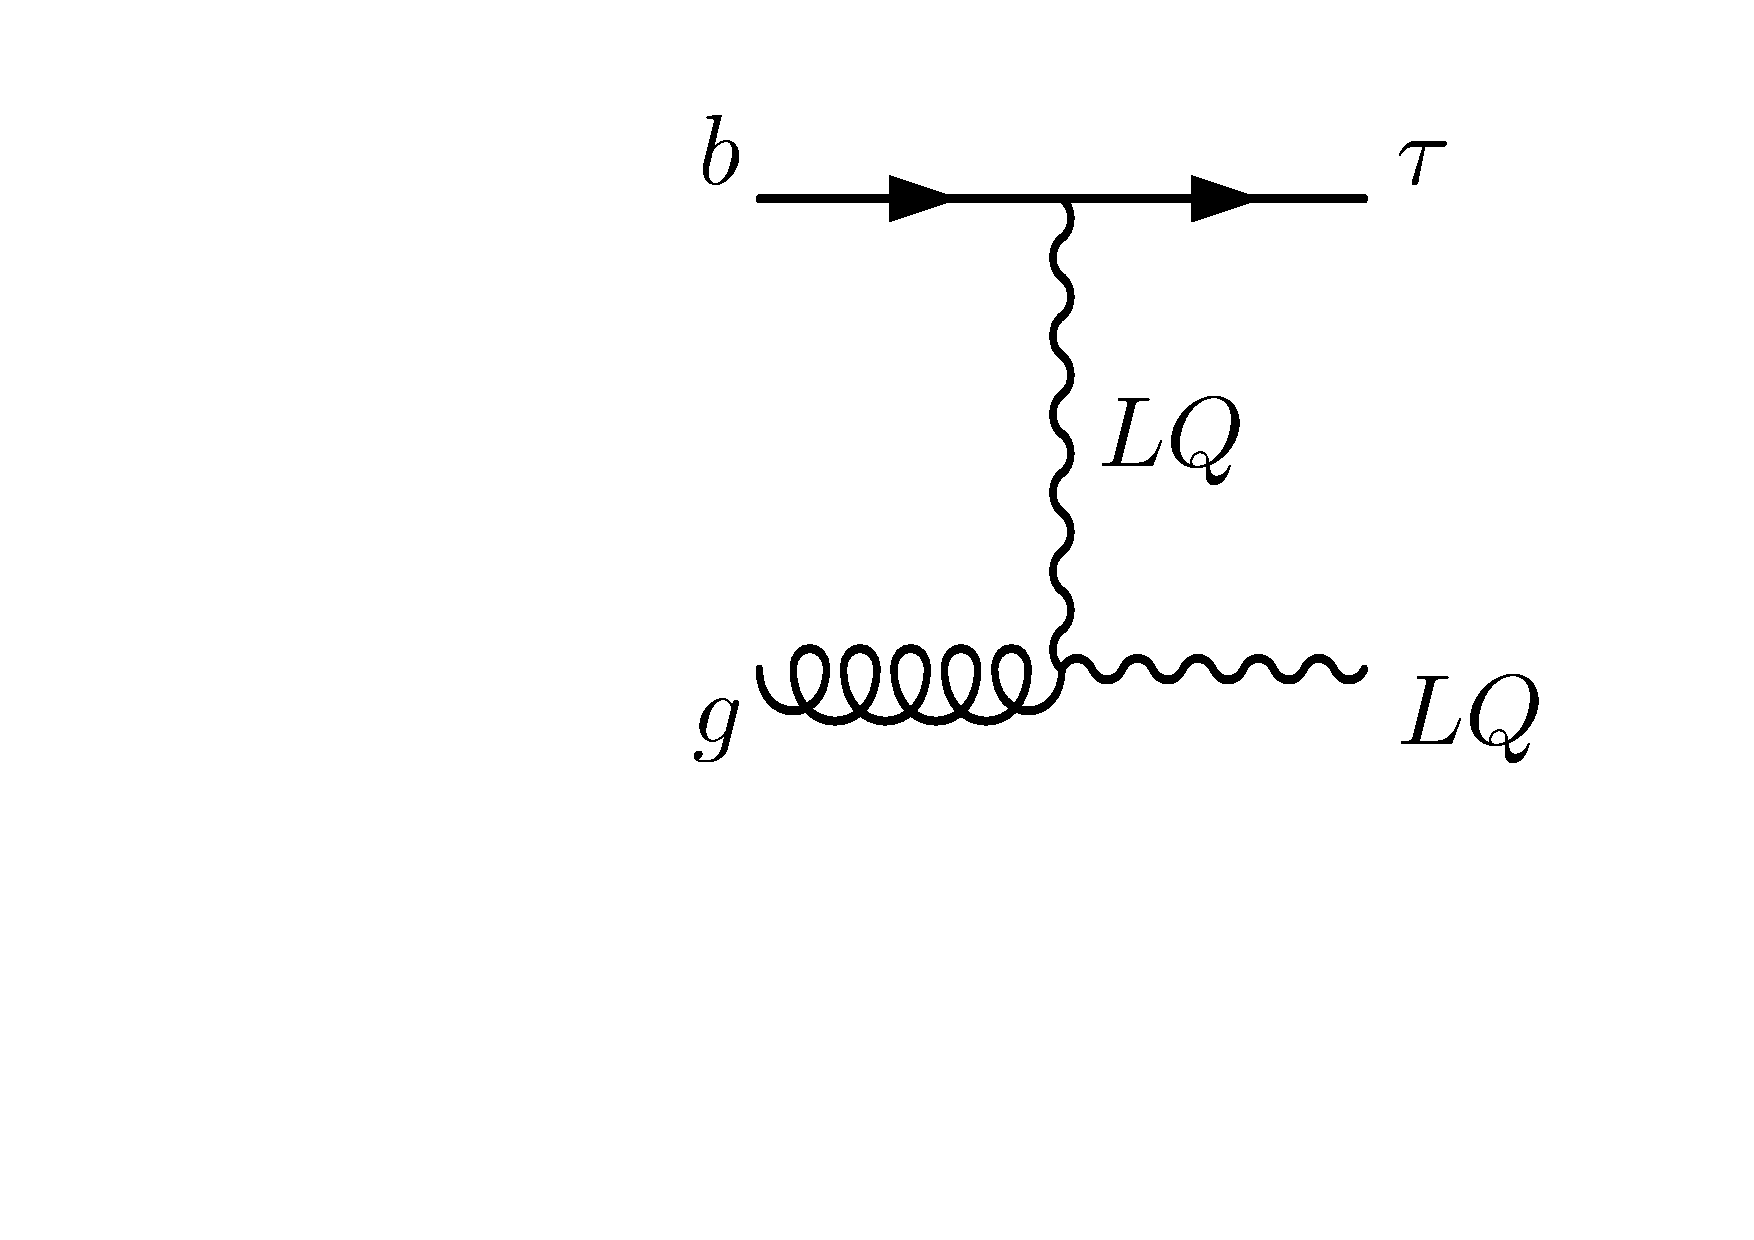
\includegraphics[width = 1.1\textwidth]{Images/feynman_diagrams/sLQ.pdf}
        \caption{}
    \end{subfigure}
    \hfill
    %Double Leptoquark Production Diagram
    \begin{subfigure}[b]{0.32\textwidth}
        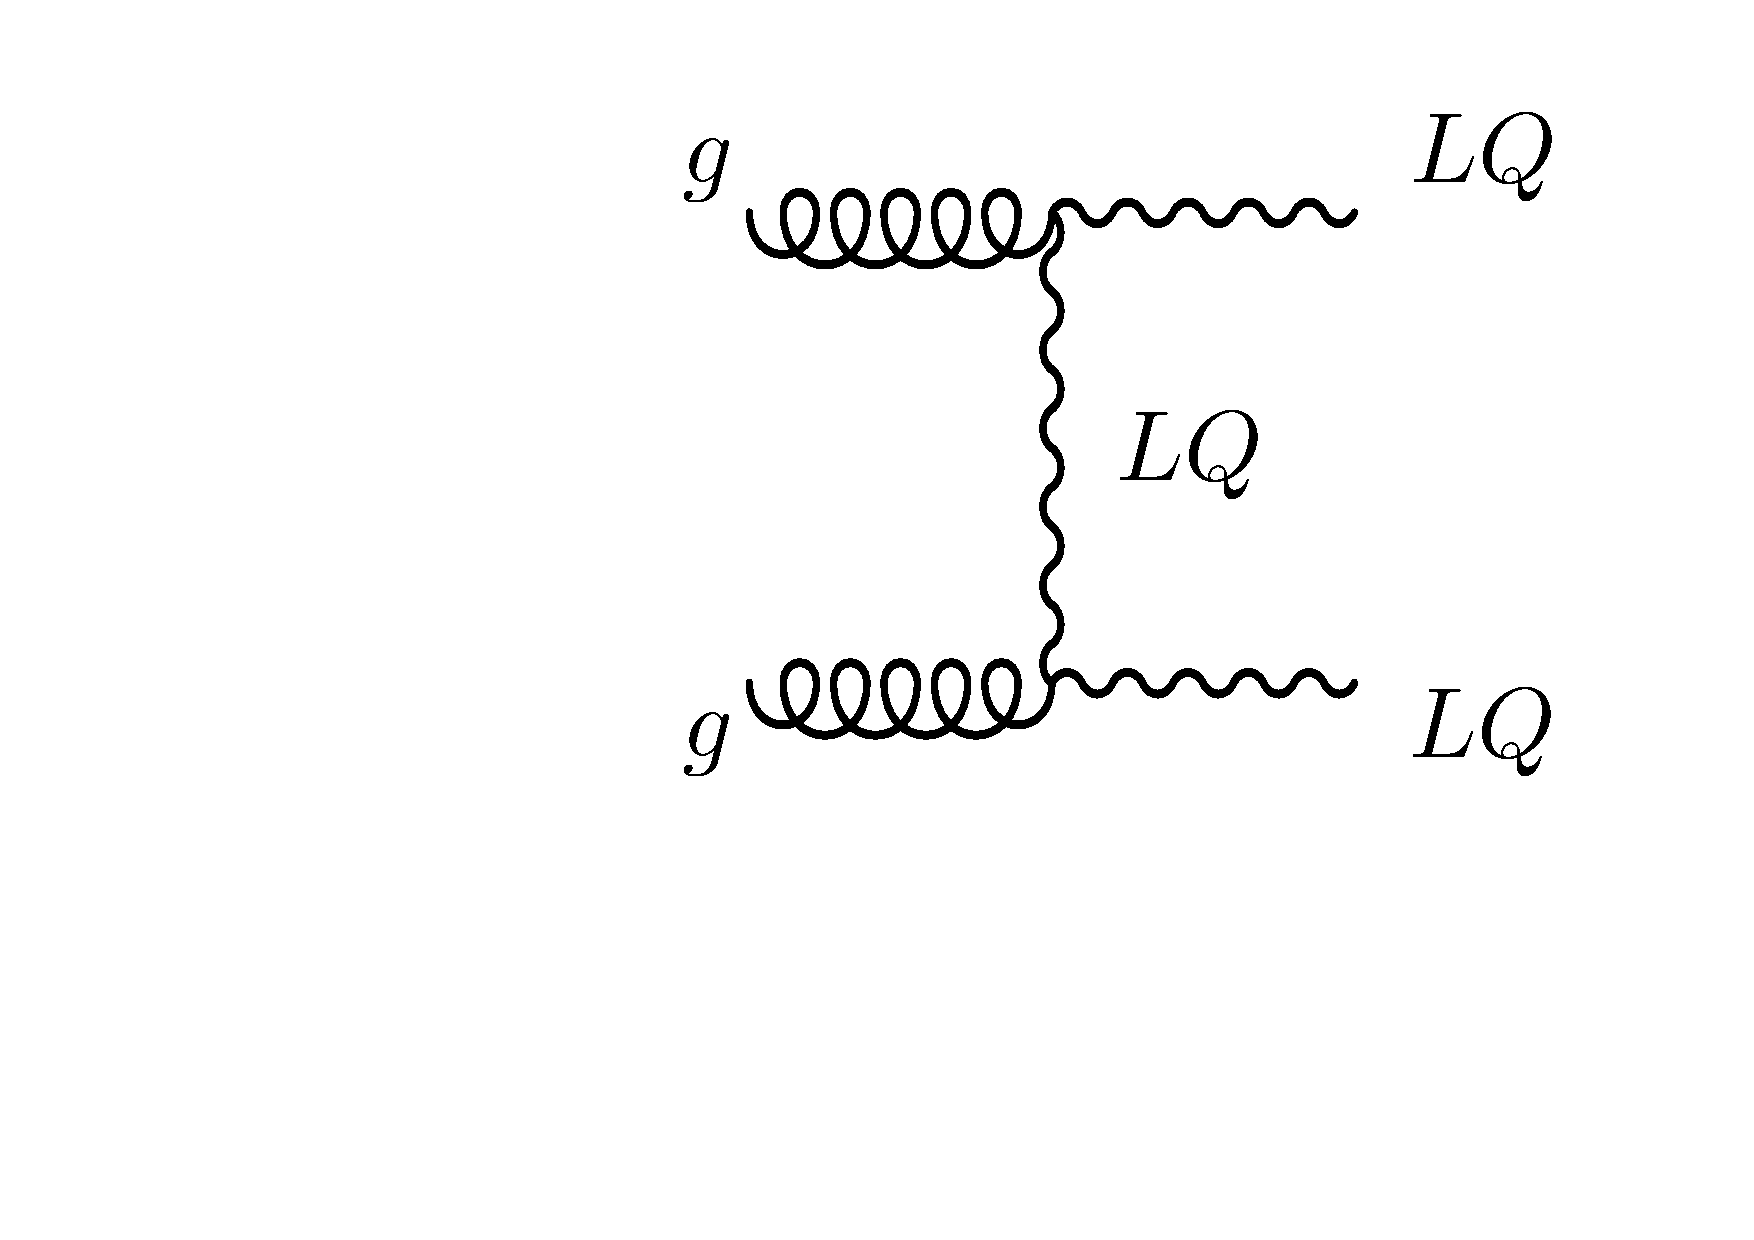
\includegraphics[width =  1.1\textwidth]{Images/feynman_diagrams/dLQ.pdf}
        \caption{}
    \end{subfigure}
    \hfill
    %non-resonant Leptoquark mediation Diagram
    \begin{subfigure}[b]{0.32\textwidth}
        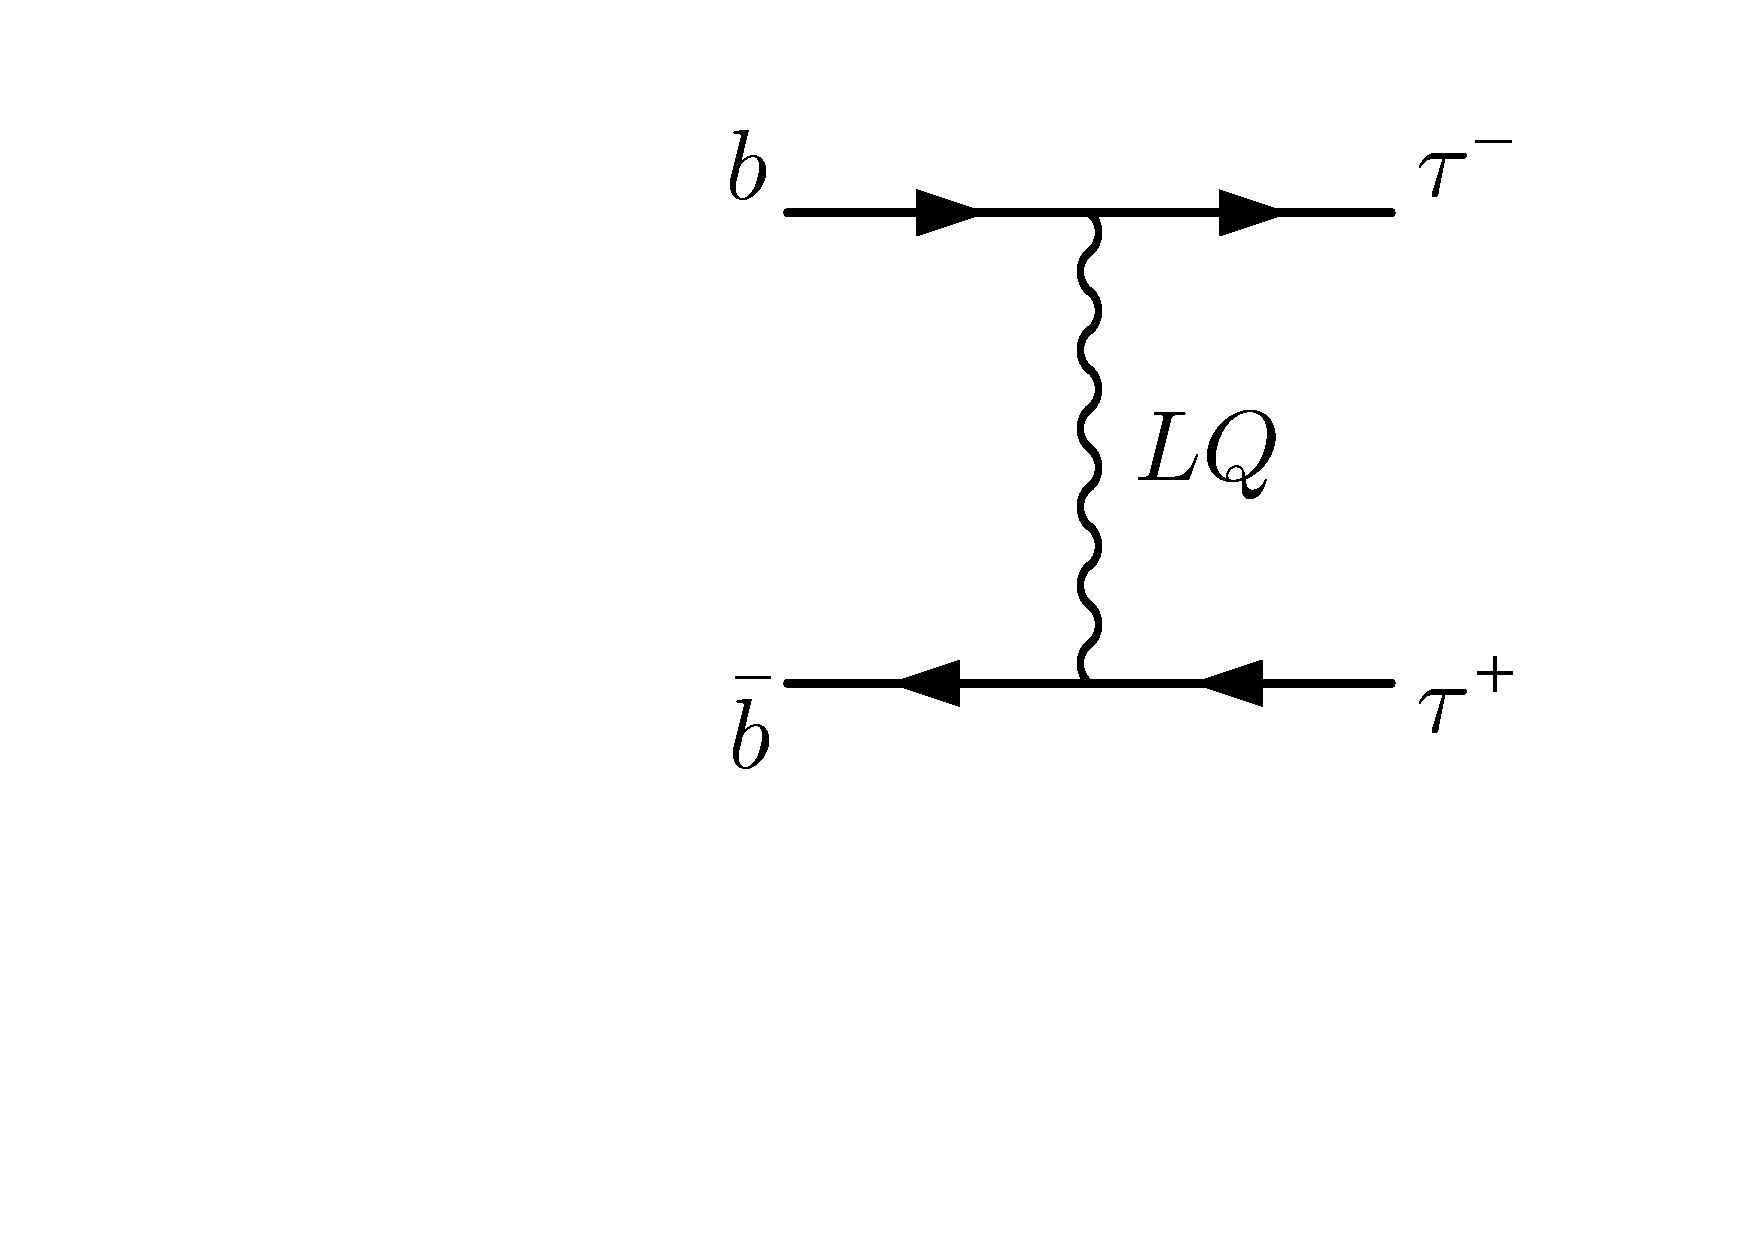
\includegraphics[width =  1.1\textwidth]{Images/feynman_diagrams/non_res.pdf}
        \caption{}
    \end{subfigure}
    \caption{Representative Feynman diagrams of single (a), pair  (b), and non-resonant (c) production leptoquarks in proton-proton collision experiments. In single and pair production, the diagrams shown involve t-channel LQ exchange, dominant for lower LQ mass. However, for larger mass there exist s-channel diagrams featuring a virtual bottom quark and gluon, respectively.}
    \label{fig:feynmp-prod-channels}
\end{figure}

Of the searches above, we find~\cite{CMS:2020wzx} particularly interesting. Here, the CMS collaboration explores signals corresponding to $\tq\,\nu\,\bq\,\tau$ and $\tq\,\nu\,\tau$ final states, with $137 \fb^{-1}$ of proton-proton ($\mathrm{p}\,\mathrm{p}$) collision data. The former is motivated by $\lq$ pair production, with one $\lq$ decaying into $\tq\,\nu$ and the other into $\bq\,\tau$, while the latter arises from a single $\lq$ produced in association with a $\tau$, with a subsequent $\lq$ decay into $\tq\,\nu$ (see Figure~\ref{fig:feynmp-prod-channels} for the corresponding diagrams). From the combination of both production channels, the search excludes $U_1$ masses under $1.3-1.7 \tev$, with this range depending on the $U_1$ coupling to gluons and on its coupling $g_U$ in the $\bq_L\,\tau_L$ vertex.

What makes this search particularly attractive is that, for the first time, an LHC collaboration directly places (mass dependent) bounds on $g_U$. This is important, since having information on this parameter is crucial in order to understand if the $U_1$ is really responsible for the $R_{D^{(*)}}$ anomaly. The inclusion of the single-$\lq$ production mode is important, since its cross-section is directly proportional to $g^2_U$. However, as can be seen in Figure~6 of~\cite{CMS:2020wzx}, the current constraints are dominated by pair production, with single-$\lq$ production playing a subleading role. While this is expected~\cite{Schmaltz:2018nls}, it still leads us to ponder the possibility of improving the sensitivity of LHC searches to single-$\lq$ production, and thus on achieving better constraints on $g_U$. Other complementary and similar searches to~\cite{CMS:2020wzx} were carried out by both ATLAS~\cite{ATLAS_7A} and CMS~\cite{LQS_CMS_2022_results_comparison}.

It is also well known, though, that searches for an excess in the high-$\pt$ tails of $\tau$ lepton distributions can strongly probe $g_U$, up to very large $\lq$ masses. Indeed, as shown in~\cite{Faroughy:2016osc,GINO_2022}, the new physics effective operators contributing to $R_D{^{(*)}}$ also contribute to an enhancement in the $\mathrm{p}\,\mathrm{p}\to\tau\tau$ production rates. This has motivated a large number of recasts~\cite{Angelescu:2018tyl,Schmaltz:2018nls,Baker:2019sli,Bhaskar:2021pml,Angelescu:2021lln,Cornella:2021sby,Allwicher:2022gkm,Haisch:2022afh,GINO_2022}, as well as a CMS search explicitly providing constraints in terms of $U_1$~\cite{CMS:2022goy}. Nevertheless, it is important to note that for these $\mathrm{p}\,\mathrm{p}\to\tau\tau$ processes, the $\lq$ participates non-resonantly, so contributions to the $\mathrm{p}\,\mathrm{p}\to\tau\tau$ rates and kinematic distributions from non-LQ BSM diagrams containing possible virtual particles, such as a heavy neutral vector boson $\zb'$, could spoil a straightforward interpretation of any possible excess~\cite{Baker:2019sli}. Thus, it is also necessary to understand how the presence of other virtual particles can affect the sensitivity of an analysis probing $g_U$.

In this work we study the projected $\lq$ sensitivity at the LHC, considering already available $\mathrm{p}\,\mathrm{p}$ data as well as the expected amount of data to be acquired during the High-Luminosity LHC (HL-LHC) runs. We explore a proposed analysis strategy which utilizes a combination of single-, double-, and non-resonant-LQ production, targeting  final states with varying $\tau$-lepton and b-jet multiplicities. 
The studies are performed considering various benchmark scenarios for different $\lq$ masses and couplings, also taking into account distinct chiralities for the third-generation fermions in the $\lq$ vertex. We also assess the impact of a companion $\zb'$, which is typical of gauge models, in non-resonant $\lq$ probes, and find that interference effects can have a significant effect on the discovery reach. We consider this effect to be of high interest, given that non-resonant $\lq$ production can have the largest cross-section, and thus could be an important channel in terms of discovery potential.

An important aspect of this work is that the analysis strategy is developed using a machine learning (ML) algorithm based on Boosted Decision Trees (BDT)\cite{friedman_greedy_2001}. The output of the event classifier is used  to perform a profile-binned likelihood test to extract the overall signal significance for each model considered in the analysis. The advantage of using BDTs and other ML algorithms has been demonstrated in several experimental and phenomenological studies~\cite{Ai:2022qvs,Biswas:2018snp,ATLAS:2017fak,Chigusa:2022svv,Chung:2020ysf,Feng:2021eke,ttZprime}. In our studies, we find that the BDT algorithm gives sizeable improvement in signal significance.
